\scanpage{27}

cette dernière relation $\Sigma_1^-\cap\Sigma_2^-\ne\varnothing$ est vraie $=$ si $E_1=E_2=\varnothing$, car \deleted{\unsure{donc|alors} par hyp.} si on avait de plus $\Sigma_1^-\cap\Sigma_2^-=\varnothing$, on en conclurait que les deux \deleted{part.} décompositions binaires \deleted{\unsure{son|sont}} (qui sont alors des partitions binaires) sont \uline{identiques}, ce que l'on \inserted{a} exclu. Cela montre que les $\Sigma_1^+,\Sigma_2^+$ sont uniquement déterminés.

On a donc le diagramme d'inclusions
\diagram{\begin{tikzcd}[ampersand replacement=\&,column sep=small]
\Sigma_1^+ \& E_1 \arrow[l,hook] \arrow[r,hook] \& \Sigma_{12} \& E_2 \arrow[l,hook] \arrow[r,hook] \& \Sigma_2^+
\end{tikzcd}}
qu'on, exprime par un diagramme
\figure{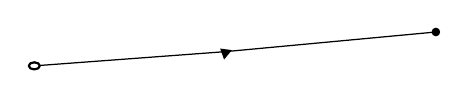
\begin{tikzpicture}[x=1cm,y=1cm,line cap=round,line join=round]
\draw[line width=.45pt] (0,0) -- (2.42,.18) -- (5.1,.43);
\draw[line width=.8pt,fill=white] (0,0) ellipse (.07 and .045);
\fill (2.36,.22) -- (2.51,.20) -- (2.41,.08) -- cycle;
\fill (5.1,.43) circle (.055);
\end{tikzpicture}}
% The following inclusion chain is the written label immediately below the drawing.
\diagram{\begin{tikzcd}[ampersand replacement=\&,column sep=small]
\Sigma_1^+ \& E_1 \arrow[l,hook] \arrow[r,hook] \& \Sigma_{12} \& E_2 \arrow[l,hook] \arrow[r,hook] \& \Sigma_2^+
\end{tikzcd}}
\margin{\[
\text{NB}\left\{\begin{aligned}
\Sigma_1^-&=\Sigma_{12}\amalg_{E_2}\Sigma_2^+\\
\Sigma_{\deleted{\unsure{1}}2}^-&=\deleted{E}\Sigma_{12}\amalg_{E_1}\Sigma_1^+
\end{aligned}\right.
\]}

\margin{Ceci n'implique pas que les quatre ensembles $\Sigma_1^+,\Sigma_1^-,\Sigma_2^+,\Sigma_2^-$ soient distincts, car on peut avoir (\unsure{bien pas|non pas} $\Sigma_1^+=\Sigma_2^+$, ni $\Sigma_1^-=\Sigma_2^-$, mais) $\Sigma_1^+=\Sigma_2^-$, qui équivaut à $E_1=\Sigma_{12}$ et entraîne $E_2=\varnothing$ (Cela signifie, en termes des $(\Sigma_{\unsure{1|t}}^+,\Sigma_1^-)$ que $\Sigma_2^{\unsure{\dot{-}|-}}=\Sigma_1^+$, $\Sigma_2^+=X\setminus\Sigma_1^+=\overset{\leftarrow}{\Sigma}{}_1^{-,\unsure{\circ|0}}$) \deleted{ou} et la relation \unsure{symetrique|symétrique}. On ne veut pas exclure ce cas, i.e.\ \deleted{\unsure{nous|mais}} n'exige pas que les quatre ensembles $\Sigma_1^+,\Sigma_1^-,\Sigma_2^+,\Sigma_2^-$ soient distincts s'ils le \unsure{\deleted{sont}|sont}, \unsure{on|c.-à-d.} dit que les \deleted{ens.} \inserted{deux décomp. bin.} \deleted{\unsure{sont strictmt}} \unsure{non parallèles|sont non parallèles}.}

Je me propose d'étudier les ensembles finis \unsure{indicellés|indiciellés} $\deleted{\unsure{\Pi|\Sigma}}(\unsure{\pi|\Pi}_\alpha)_{\alpha\in A}\deleted{=(\Sigma_\alpha^i),\unsure{\alpha\in A}}$ $\deleted{\pi_\alpha=\{\Sigma_\alpha^\varepsilon}$ de décompositions binaires de $\unsure{X}$ deux à deux non parallèles.

Voici une façon très \unsure{générale|génerale} d'\deleted{en}obtenir des \unsure{floppées|floppés}.

% archive sheet number: 26
